\documentclass{article}
\usepackage{multicol, lineno, parskip, graphicx, subcaption, listings}

\title{%
Chop Chop \\
  \large Group Report}
\author{
  Connor, Wood\\
  \texttt{cw668}
  \and
  Will, Haysom\\
  \texttt{wah20}
  \and
  Dean, Gooding\\
  \texttt{Dmag2}
  \and
  Beth, Hill\\
  \texttt{Berh2}
  \and
  Jack, Fermer\\
  \texttt{Jf500}
}

\begin{document}

\maketitle

\pagebreak

\pagenumbering{roman}
\linenumbers

\begin{abstract}
  \addcontentsline{toc}{section}{Abstract}
      This report surrounds our group software development project, a smart cooking assistant called \emph{Chop Chop}. 
    
      In this report we will showcase our group project. We will be evaluating not only the software we made but also how we made it, looking into our design, development, and ways of working.

      We work through this report in a semi-chronological order. We first outline our research and aims. We will later use our aims as metrics to critique how well we acheived our goals. We then explain how we made Chop-Chop, and go on to discuss what we could have done with more time.

      Throughout the report we will explain both the acheivements and pitfalls we have fallen into as a group and how we dealt with them.
  \end{abstract}

  \pagebreak

  \tableofcontents

  \pagebreak

  \pagenumbering{arabic}

  %\begin{multicols}{2}

    \section{Introduction}
Chop Chop makes cooking more accessible by offering hands-free, smart recipes. Our smart recipes allow users to cook without having to worry about looking through the steps of a recipe, scrolling a screen with messy hands, or starting timers. It achieves this by using a convoluted neural network (CNN), computer vision, and a full-stack application.

We made this application as a team of five people, all with previous experience of developing on large projects. Following agile methodologies, we used our experience and finished our development with a prototype of a full-stack application which achieves what we set out to do. 

We implemented extra features on our project which we did not plan to do when the project was defined. Conversely, we ran into some problems which meant we had to adapt some aspects of the original plan.

    

    \section{Aims}
We decided on these objectives to measure our progress and ensure a clear direction preventing any feature creeping. Additionally, we identified stretch objectives to achieve in case we have additional time at the end of the project
\subsection{Objectives}
\begin{itemize}
  \item {Front-end electron application for users to display each recipe step}
  \item {Ability to search, create, view and favourite pre-written recipes.}
  \item {Create a dataset to recognise at least enough ingredients for one recipe}
  \item {AI to recognise the completion of steps using image recognition with cameras so that we progress the recipe automatically.}
  \item {Ability for users to manually progress recipe steps using buttons to progress or go back if the AI has incorrectly marked a step as completed.}
  \item { Complete one full recipe run-through on a complex dish}
\end{itemize}
\subsection{Stretch Objectives }
\begin{itemize}
  \item {Voices to read recipe steps out loud.}
  \item {Simple IoT \footnote{Internet of Things} integrations.(e.g use raspberry pi)}
  \item { Additional ability for the AI to recognise events such as pasta boiling over and display warning steps on the user’s device}
\end{itemize}
    \section{Ways of Working}
    \subsection{User Stories}
    Right at the start of our project, we came up with and decided on our user stories. We took our vision of what a theoretical end-product would be. It was broken into fundamental statements that the user should “feel” when they use the product. Below we state the story, then the features it will need.

    \begin{center}
        \textbf{\textit{“I should be able to progress a recipe without touching the screen”}}
        \begin{itemize}
            \item A Camera rig system to observe the kitchen's working areas.
            \item Object detection system that tells us what’s in the camera's frames. 
            \item System to check if the culinary objects present satisfy the recipe step.
            \item Way to send the correct step to a GUI.
        \end{itemize}
        
        \textbf{\textit{“It should be clear to the user what to do for each step”}}
        \begin{itemize}
            \item Design with thought and simplicity in mind.
        \end{itemize}
        \textbf{\textit{“UI Should be easy to use and modern”}}
        \begin{itemize}
            \item UI should be intuitive and follow common design protocols.
        \end{itemize}
        
        \textbf{\textit{“Our interface should be accessible for a range of different disabilities”}}
        \begin{itemize}
            \item Design a colour palette that is easy to see and offers good levels of contrast.
            \item A text-to-speech system that can verbally guide the user alongside displayed text.
        \end{itemize}
        
    \end{center}
    \subsection{Source Control}
    One of the key components to Chop-Chops’ success was our well-set-up and organised GitLab repository. 

    Initially, we decided to create a Gantt chart to record the project timeline and delegate deliverables, which was broken down into two-week sprints. Once all members approved this, it was sent to our supervisor who provided insight into improvements to ensure the project worked effectively. An example of this would be adding our module assessments to the chart to accurately manage and consider our university commitments and workload. 

    A scrum-style agile approach was adopted to our project management strategy. We broke down our Gantt charts’ deliverables into “Issues” on Gitlab. Issues were put on our virtual board, which had four categories, Open, In Development, Review/ Testing, and Closed. These issues were assigned and then moved across given their completion state. 

    From our team’s year-in-industry experience, we adopted a review before merging convention. This rule ensures that tasks were overlooked by other members before being added to the main branch from their working one. This had two main advantages. One was a hugely reduced chance of buggy code getting into the main branch. Two: you gained knowledge of how the rest of the project worked outside of your assigned issues. To enforce this, we locked the main branch from being merged and required at least one approval before the merge.

    We aimed to ensure the main branch was kept as clean as possible; we were mindful of what should and should not be on the repo. This included adding rules to the git ignore file when needed, pruning unnecessary files, and ensuring consistency in naming conventions for files and folders.

    \subsection{Meetings}
    \subsubsection{Meeting Documents}
    During our sprints, we scheduled one team meeting and one supervisor meeting each week. Ideally, we arranged the supervisor meeting to take place after the team meeting, allowing us to bring any discussions raised in the team meeting to the supervisor within the same week.
    Throughout the week a shared team document was available for any members to note down any questions or issues that they wanted to raise in the team meeting. This functioned very well as it meant discussions were not accidentally overlooked during the meeting and it also allowed other members to see the discussions points raised and prepare prior to the meeting.
    We also made use of the GitLabs issues board and our own Gannt chart to keep ourselves on schedule throughout the project. These tools allowed us to easily check what work was still outstanding for the week and compare the progress we were making to our initials estimates when starting out. As this was a particularly large project to undertake it was crucial we kept ourselves on track this way.
    \subsubsection{Team Meetings}
    At the beginning of each team meeting, we allocated a minute-taker to record the discussions. We would then begin by addressing any discussion points or questions raised in the shared document or brought up by members during the meeting. The practice of having discussions pre-documented in the shared file significantly sped up the note-taking process, enabling us to focus more on the discussions themselves. 
    Following the discussions, we would quickly cover all issues closed on the GitLabs since last meeting, making note of them in the minutes, before reviewing any outstanding issues. We made sure that each team member individually was making good progress and was clear with what work was still to be done and provided team assistance to any members that were encountering any difficulties with their work.
    Finally, we would create new issues aligned with the progress steps outlined on the Gannt Chart and assign them out to team members based on their current workloads and experience in the given areas of the project.
    \subsubsection{Supervisor Meetings}
    Our supervisor meetings were usually well organised as we would make notes during the team meetings for any discussions to be bought up to the supervisor. Any feedback or recommendations were then considered, and issues and objectives updated to reflect any changes from the meeting.
    As well as this, we made sure to keep our supervisor updated on our progress and any issues closed since the last meeting and inform them of the issues outstanding and assigned for this week. This way we made sure the supervisor was always aware of the work we were aiming to achieve for next week and could hold us accountable for any delays.


    \section{Research}
    \subsection{Object detection}
    Our project's flagship feature was our custom real-time object detection system. This would be used to detect culinary objects such as food and utensils which would dictate when a recipe step had been completed.
    
None of us on the project had experience creating an object detection system. So, we began by doing some research. 

With the huge demand for real-time object detection in the modern age many different algorithms have emerged.

Faster R-CNN offers a real-time object detection algorithm version of R-CNN. “One of the most accurate object detection algorithms” \cite{FasterRCNN} with the drawback of “requires a lot of power at inference time” IE when running in real-time. So, detecting small food objects in a kitchen would be perfect. However, we hoped to run on a Raspberry Pi (a hub in the kitchen area), and we fear the Raspberry Pi will not have the computational power required \cite{Fast-CNN-Rasberry-Pi} at inference time.

Detectron2- Created by Facebook AI research it claims to “provides state-of-the-art detection and segmentation algorithms” \cite{wu2019detectron2} and has been used in many Facebook products such as “Smart Camera for new Portal video-calling devices” \cite{metasmartcameras}. It’s built using the COCO, LVIS, CityScape, and VOC20 datasets, this creates an accurate dataset with an MNAP. However, in many cases “YOLOv8 models outperformed the detectron2 mode” \cite{ai5010005}.

YOLO – You Only Look Once, “It is a state-of-the-art, real-time object detection system which offers extreme levels of speed and accuracy.” \cite{rajeshwari2019object}, that is around “1000x faster than RCNN and 100x faster than the Fast R-CNN model” \cite{rajeshwari2019object}.  It's also shown to have a much higher mAP50-95 "96.7\%" compared to detectron2 (Faster RCNN-101) at "83.554\%" \cite{ai5010005}.

Dean reached out to an ex-colleague who had experience in this area. They suggested using YOLOv8 \cite{Jocher_Ultralytics_YOLO_2023} as a base for real-time object detection and suggested using Roboflow \cite{RoboFlow-Software} for dataset management. 

RoboFlow \cite{RoboFlow-Software} is a site where you can easily collaboratively create image datasets. It allows you to upload images you have taken for training, delegate annotation jobs out to different members of the team, and then create a dataset which can be downloaded and trained locally. It was one of the few sites that offered an immense data set (max 10,000 images) with an easy-to-use interface, all for free.

During our research process, we tried out Roboflow and used a trial of their training cloud computers. With only 100 images we were able to confidently detect a Rubik's cube, being held, rotated in the hand, and placed under different backgrounds. Given the lack of experience we had, the relatively small number of images, and the very accurate results we achieved. We were confident that scaling up to whole recipes should on paper be very possible.
    
\section{Design}
\subsection{Frontend}
Figma was the main tool which we used to craft the frontend design of our web application. We were able to create and pull ideas from each other and prototype how we wanted the design of the application to look by using its collaborative interface. Within this section, we outline our process of exploring and integrating various ideas into our designs, as well as how we utilised Figma to translate these designs into functional code.

\subsubsection{Research}

Our design process began by investigating and researching what other recipe applications offered in terms of layout, features, and user experience. The three main recipe applications which we focused our research on was BBC Good Foods, AllRecipes and Yummly. 

\paragraph{Featured Recipe}
Our findings found that the majority of the sites that we looked at showed a featured article or recipe which was the the forefront of the homepage. This component would usually include a background image, title, description, and a button directing users to the featured collection. We quite liked this idea, as it was visually appealing, and an effective way to draw users attention to a focal point on the homepage. We also liked how it could streamline user navigation, and that we could implement our own functionality to make the component work well with our application.

\begin{figure}[h]
  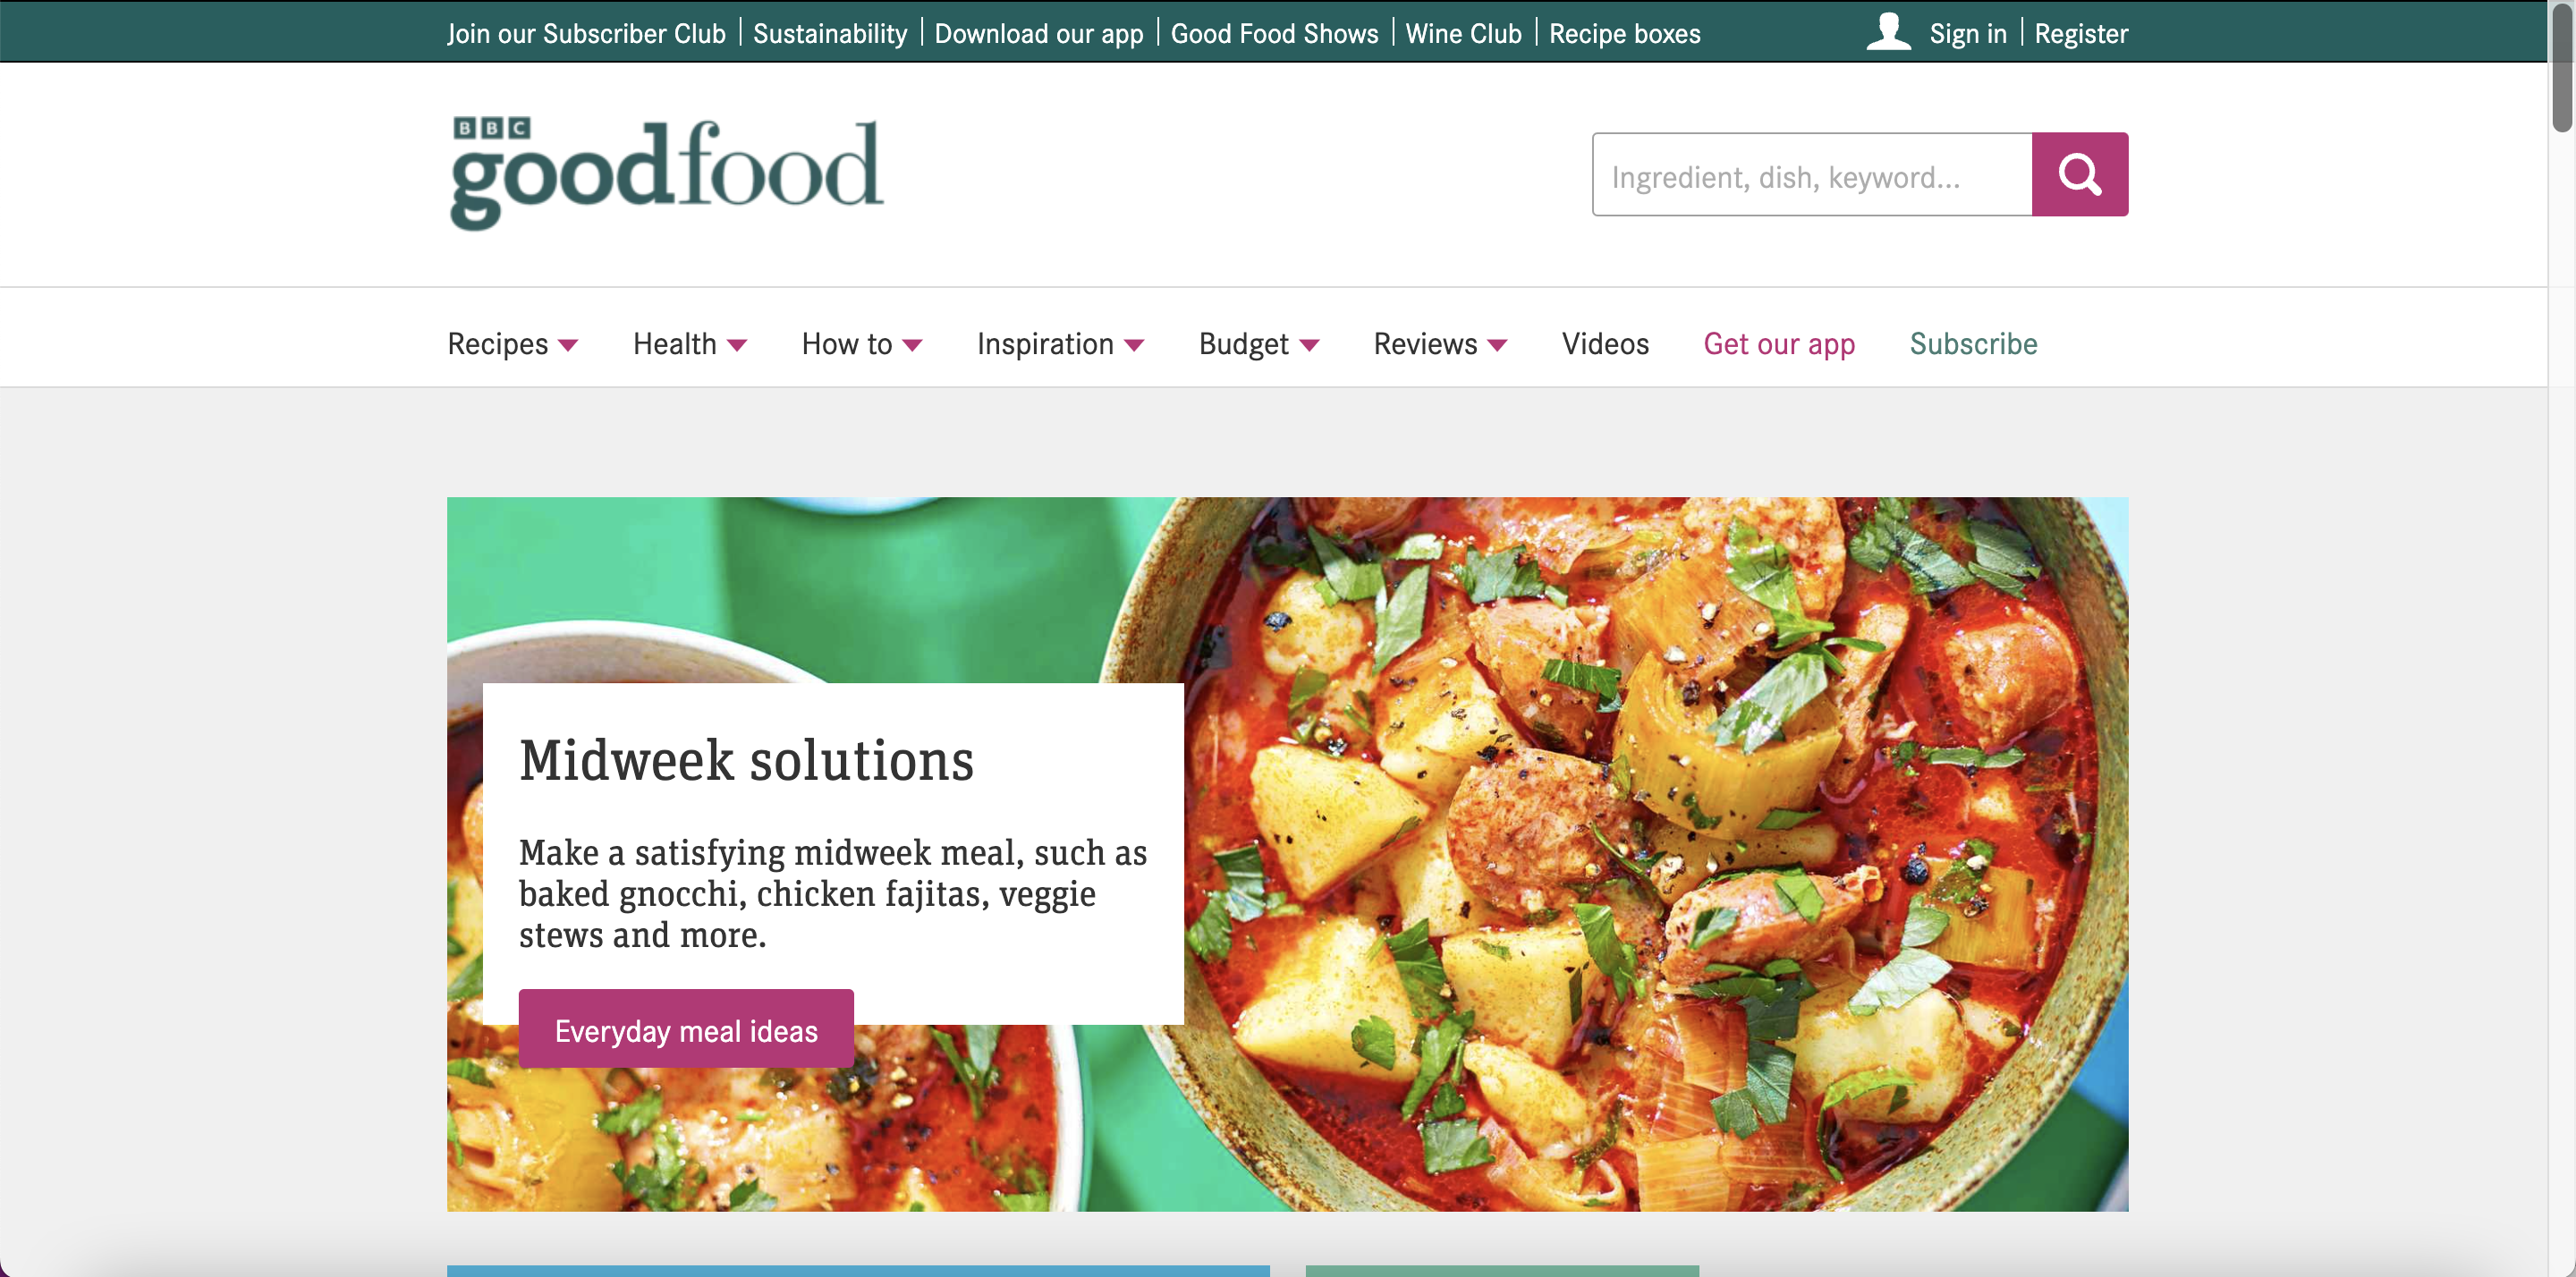
\includegraphics[width=1.0\textwidth]{assets/design-images/BBCGF featured-image.png}
  \centering
  \caption{Homepage featured article shown on BBCGoodFoods}
\end{figure}

\paragraph{Recipe cards}
Each site also used cards as a way to display each recipe. We found that this was an effective way to display each of the recipes, while only showing the necessary information needed for the user.

On Yummly, a variation of their recipe cards caught our attention with an interactive hover feature. Initially displaying just the recipe title, hovering over the card revealed more details about the recipe. We aimed to incorporate a similar functionality into our own cards.

\begin{figure}[h]
  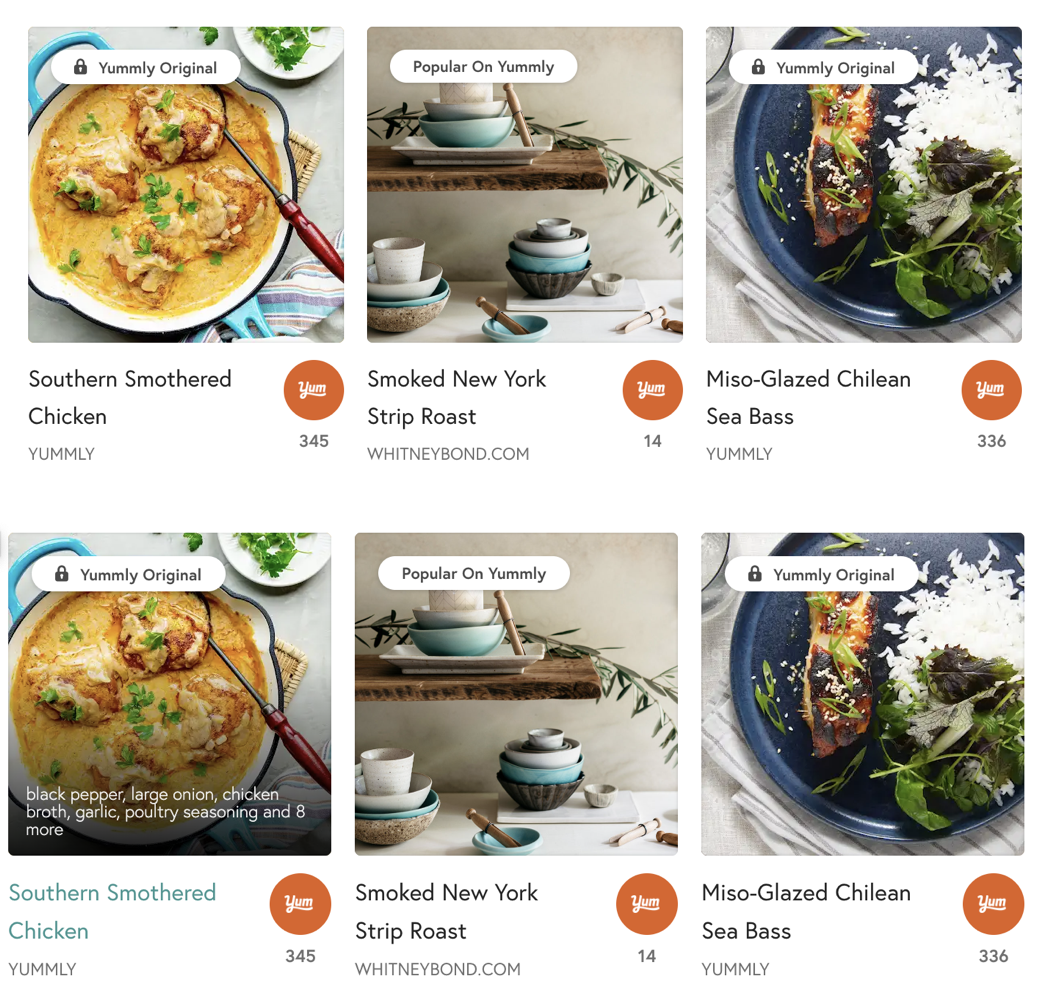
\includegraphics[width=1.0\textwidth]{assets/design-images/Yummly recipe cards.png}
  \centering
  \caption{Recipe cards featured on Yummly}
\end{figure}

\paragraph{Recipe Overview}
For the Recipe Overview page, we wanted the user to be able to see a summary of the recipe and navigate between seeing the recipe steps and the ingredients in a seamless way.

To keep the design of the page simple and clean, we split the page into two sections: the header and the information. The header of the page would show off important information about the recipe, such as the name, a description and a summary of how long the recipe will take to prepare. This section would also feature a start recipe button to take the user to the recipe carousel page.

The information section of the page would showcase both the ingredients and recipe portions of the overview.

After looking at the 3 initial sites, we discovered that the layout was overly cluttered, and the transition between viewing the recipe and its ingredients was not seamless. Instead, most sites placed the ingredients and recipe either side by side or one after the other, which disrupted the flow of navigation.

Instead, we opted for a switcher component that enables users to toggle between viewing the recipe and the ingredients. We believed that this approach would reduce clutter on the page and separate information in a more organised manner. We found inspiration for this functionality on W3Schools.

\begin{figure}[h]
  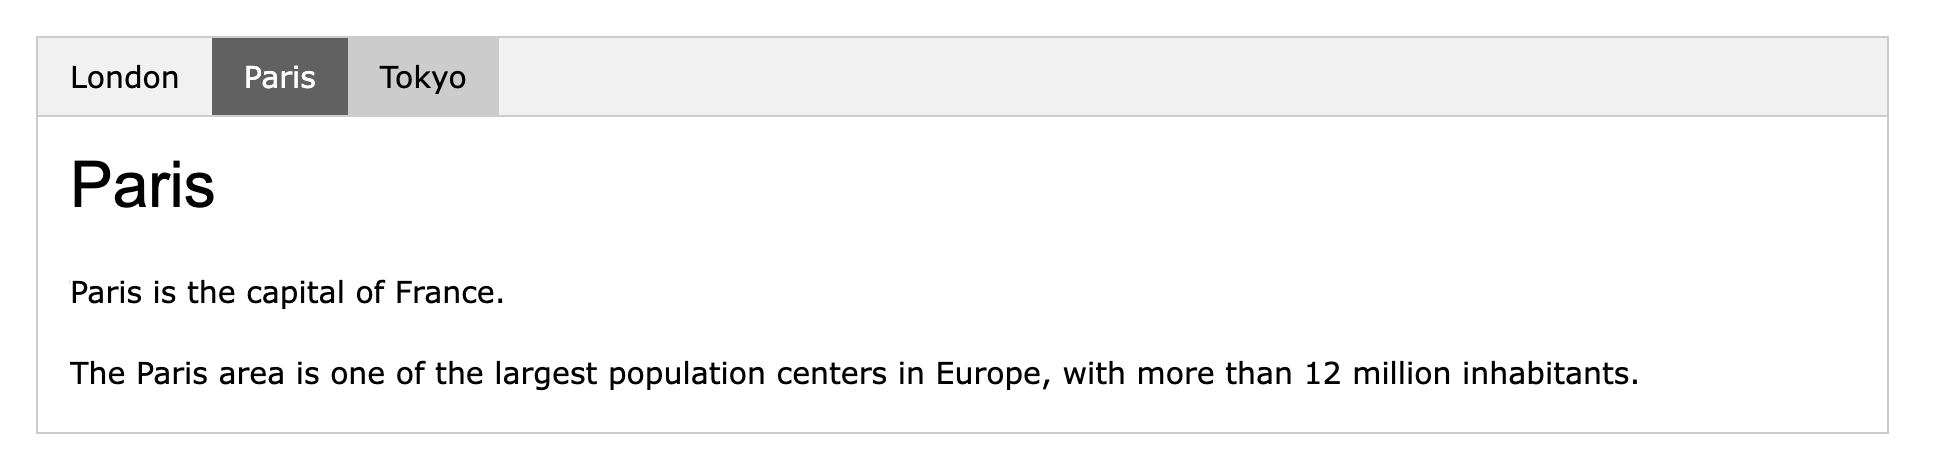
\includegraphics[width=1.0\textwidth]{assets/design-images/W3Schools tabbed component.png}
  \centering
  \caption{Tabbed component featured on W3Schools}
\end{figure}

We liked the simplicity of this design and the effective functionality to show off information without cluttering the page. 

\paragraph{Colour Palette}
To begin our investigation into which colour palette should be used for the frontend, we decided to investigate any accessibility issues which we will have to take in to consideration to ensure that our design enhanced readability and usability for all users. 

During this investigation, we found that the use of bright colours may cause pain for those who suffer with low vision or dyslexia, and may also prevent them from being able to read information from the page. This means that websites need to have a low brightness background to accommodate for this disability.

Users also need a high contrast between the text and the background on a page. According to the W3C accessibility standards, people will be able to read information better on a page which incorporates dark text on a light background. We wanted to select colours for our frontend which would meet both of these accessibility criteria and found that a neutral tone for our main colour scheme would effectively meet these standards.

For the background of the the web application, we opted to use a pale peach colour. We selected this colour as it would provide a warmth to the page while also ensuring that users who struggle with bright backgrounds are not overwhelmed when reading information. Furthermore, the selection of this colour made it easier to find secondary colours for text and highlights that would provide a bold contrast.

\subsubsection{Figma vs Zeplin}
Before we began to design the prototype of the frontend, we had to decide which software application we should use. From prior experience during our placement year, we initially chose to use either Figma or Zeplin.

Within our research, we found that Zeplin is primarily a collaboration and handoff tool whereas Figma is a comprehensive design tool that enables collaborative design, prototyping, and sharing within a single platform. This means that you could create designs directly using Figma, while on Zeplin, designs must be created using a dedicated design tool such as Sketch or Adobe XD, and then imported. 

Figma also features a Dev Mode interface that allows for developers to translate created designs into code more efficiently. As a team, we liked the use of this feature since we would be able to streamline the design-to-development workflow and reduce the use of repetitive, manual coding.

While Zeplin does also feature some developer tools, Figma is exclusively tailored for the design process. This means that Figma can provide a better experience while designing prototypes as it doe not have the additional complexity of features which are shown within Zeplin. 

After considering the pros and cons of both applications, combined with the research which we conducted, we decided that Figma would be the best solution for us.

\subsubsection{Designs: Version 1}
The initial iteration of the designs prioritised the application's functionality over user experience considerations. Inspired by our research, we designed our own components, recipe cards and recipe pages. Within this subsection, we provide a detailed description of these components and their functionalities.

\paragraph{Homepage}
We used our prior research to design a homepage which would allow the user to view and navigate to recipes easily as well as providing essential information to the user. 

Below we have highlighted the components shown within the homepage of our web application, including what each component looks like, how the components functionality works and any thoughts which we discussed to make our design improved.

\paragraph{Featured Recipe}
In designing this component, the goal was to create a visually appealing design which allowed the user to see a summarised recipe while also not making the homepage cluttered.

\begin{figure}[h]
  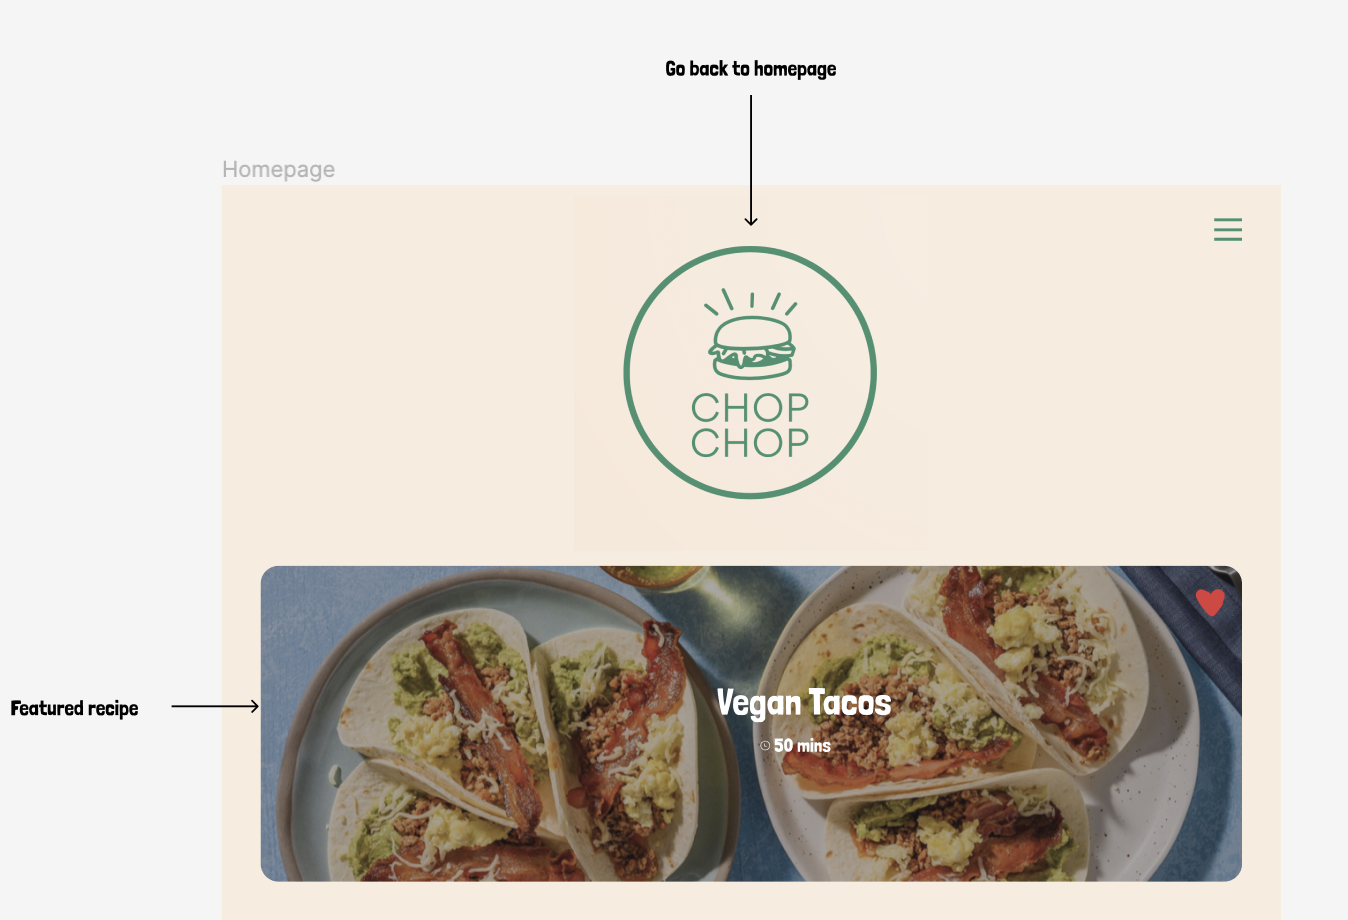
\includegraphics[width=1.0\textwidth]{assets/design-images/Version 1 Featured Recipe.png}
  \centering
  \caption{Featured Recipe component design}
\end{figure}

We designed the component so it would include a background image of the recipe, a title and some metadata including the prep and cook time of the recipe. We felt that this would still make the design eye-catching to the user, while also not overwhelming the user with information.

We wanted to make the functionality of this component randomly choose a recipe from the database, ensuring a dynamic and fresh experience for users with each visit to the homepage.

The component would also a feature a favourite button, giving the users an opportunity to save the recipe so they can build a collection of recipes which they would can go back to and find more easily in the future. 

\paragraph{Recent Recipes}  
Within the design, we wanted to add a component to show recent recipes which the user has visited before. This feature does not only allow users to revisit recipes which they may have liked before, but it also enhances the users browsing experience since users can quickly see recipes without having to search for them again, adding more simplicity and efficiency to our application.

\begin{figure}[h]
  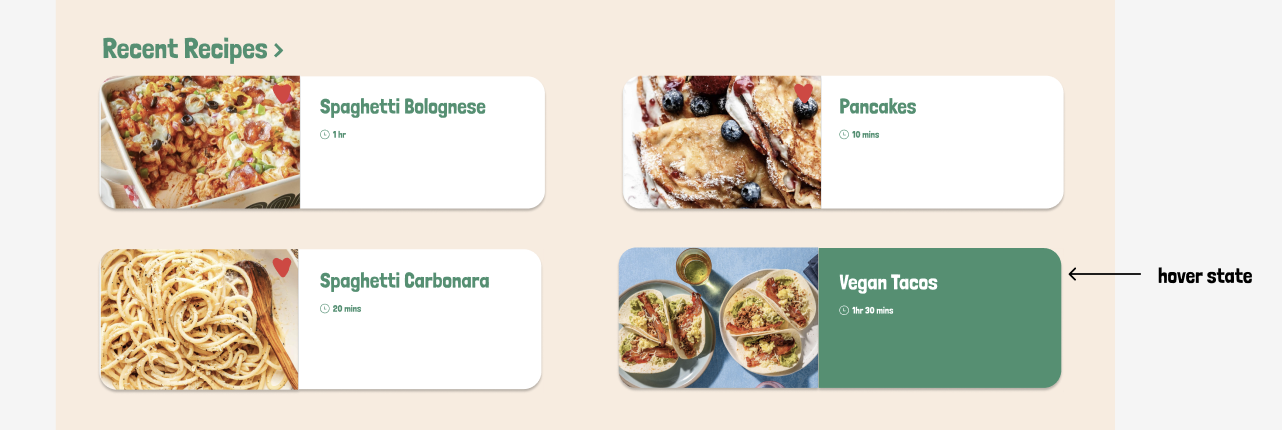
\includegraphics[width=1.0\textwidth]{assets/design-images/Version 1 Recent Recipes.png}
  \centering
  \caption{Recent Recipes component design}
\end{figure}

We liked what functionality this component could bring the our web application. By showing the user their recently viewed recipes, it would enhance user engagement and streamline their journey across the application, by allowing them to access content which they find relevant.

The design of this would include the 4 most recently viewed recipes, displayed using a card layout. We found that this layout is user friendly and visually appealing and can display each recipe in a clear and organised manner. 

\paragraph{Liked Recipes}
We also liked the idea of allowing the user to bookmark recipes which they find appealing and may want to revisit in the future. 

This feature will add another layer of personalisation for the user, allowing them to create their own collection of recipes which they may want to go back and access whenever they need them. 

\begin{figure}[h]
  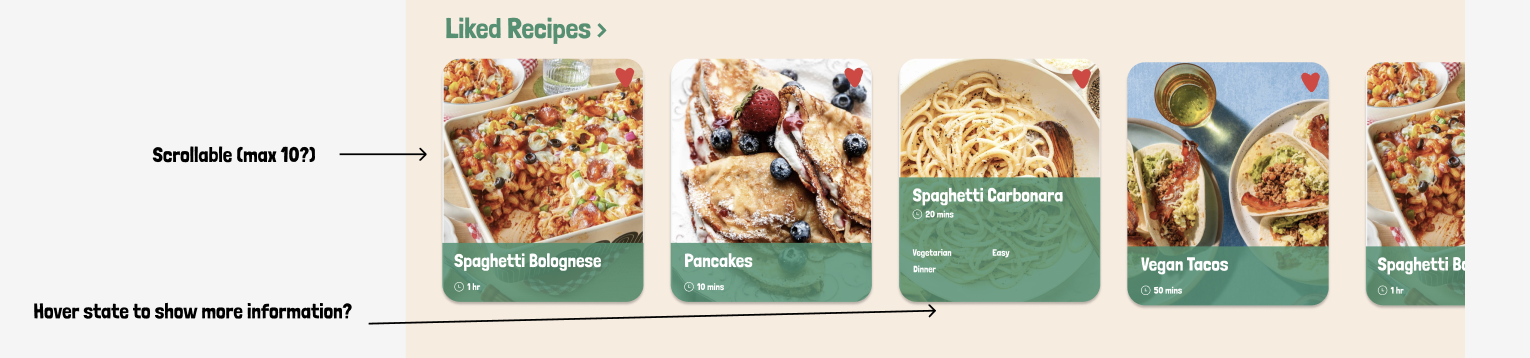
\includegraphics[width=1.0\textwidth]{assets/design-images/Version 1 Liked Recipes.png}
  \centering
  \caption{Liked Recipes component design}
\end{figure}


On each recipe card, it was designed so a heart shaped icon would be shown, providing the option for users to click and add the recipe to their liked recipe collection. 

It was designed that the component itself would feature 10 favourited recipes and a title linking the user to a search page filtered to display all their bookmarked recipes. To ensure the component would not be cluttered and overwhelming to the user, we decided that it would be best to include a scroll feature, allowing for the user to smoothly navigate though their bookmarked recipes while still providing an organised interface. 

\paragraph{Recipe Cards}
We opted to have 2 different recipe card versions within the application: horizontal and vertical. The decision to have these different types was made so the cards can be more versatile and could be used for multiple components. Both versions of the cards include an image, title, like button and some metadata to display important information to the user. 

The horizontal card has been designed to show the image of the recipe on the left-hand side, and the information associated with the recipe on the right with a white background. The vertical card was designed to have the recipe image as the background of the card, with a green box at the bottom to display the recipe information.

\begin{figure}[h]
  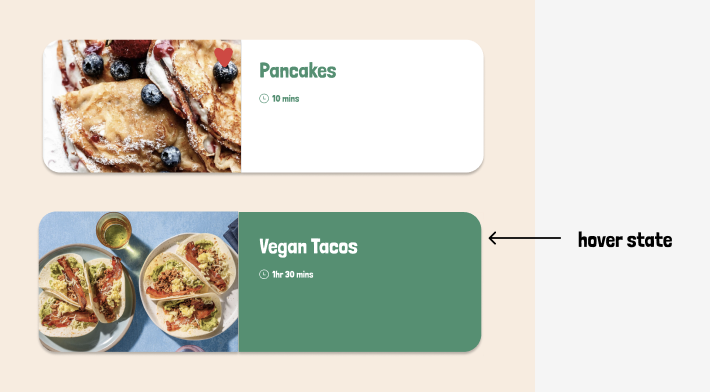
\includegraphics[width=1.0\textwidth]{assets/design-images/Version 1 Horizontal Cards.png}
  \centering
  \caption{Horizontal recipe card design}
\end{figure}

\begin{figure}[h]
  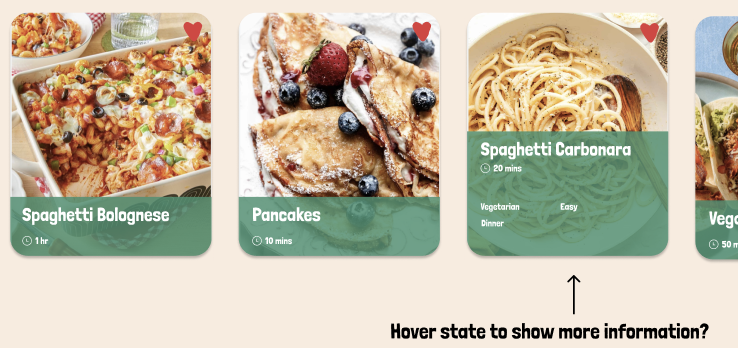
\includegraphics[width=1.0\textwidth]{assets/design-images/Version 1 Vertical Cards.png}
  \centering
  \caption{Vertical recipe card design}
\end{figure}

A hover state was also designed for each recipe card, to allow users to know which card they are currently selecting and improving accessibility. Depending on the card, different hover state versions are shown. 

Within the horizontal card, the colour scheme undergoes an inversion, with the background of the information displayed in green and the text presented in white. On the other hand, the green box displaying the recipe information within the vertical card expands and raises within the card to reveal additional details.
    
\paragraph{Recipe Overview}
The recipe overview page highlights essential elements such as ingredients, cooking steps and preparation time which allows the users to have an understanding of the recipe before they proceed with cooking.

\paragraph{Recipe Switcher}
Inspired by the W3Schools design which we saw during the research process, we decided to incorporate the recipe switcher component into the recipe overview page.

The component was designed to include two tabs which the user could switch between: Ingredients and Recipe. The ingredients section would show all ingredients which are needed for the recipe, and a checkbox to allow the user to state if the ingredients have already been prepared (e.g. carrots already being chopped). We decided to add this functionality in, as it would reduce any unnecessary steps within the recipe.

\begin{figure}[h]
  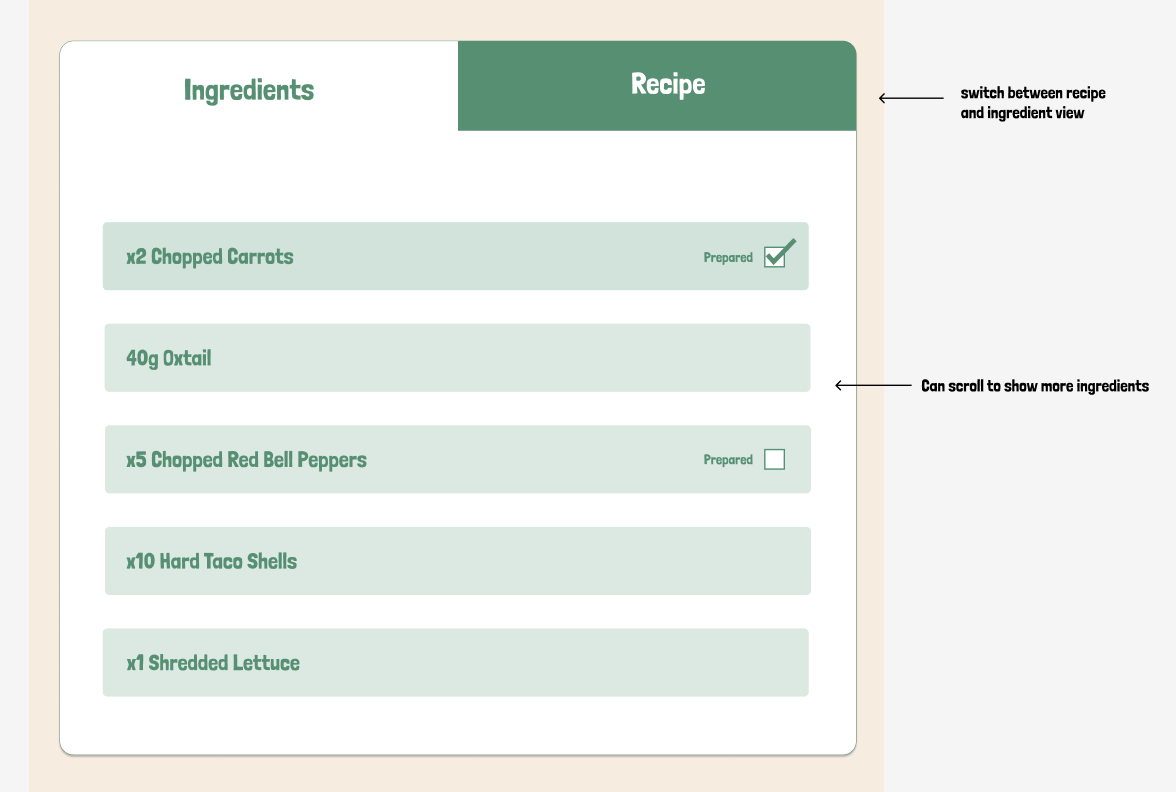
\includegraphics[width=1.0\textwidth]{assets/design-images/Version 1 Recipe Switcher ingredients.png}
  \centering
  \caption{Recipe Switcher component design showing ingredients}
\end{figure}

On the other hand, the recipe section stated the steps which the user would be following. 

\begin{figure}[h]
  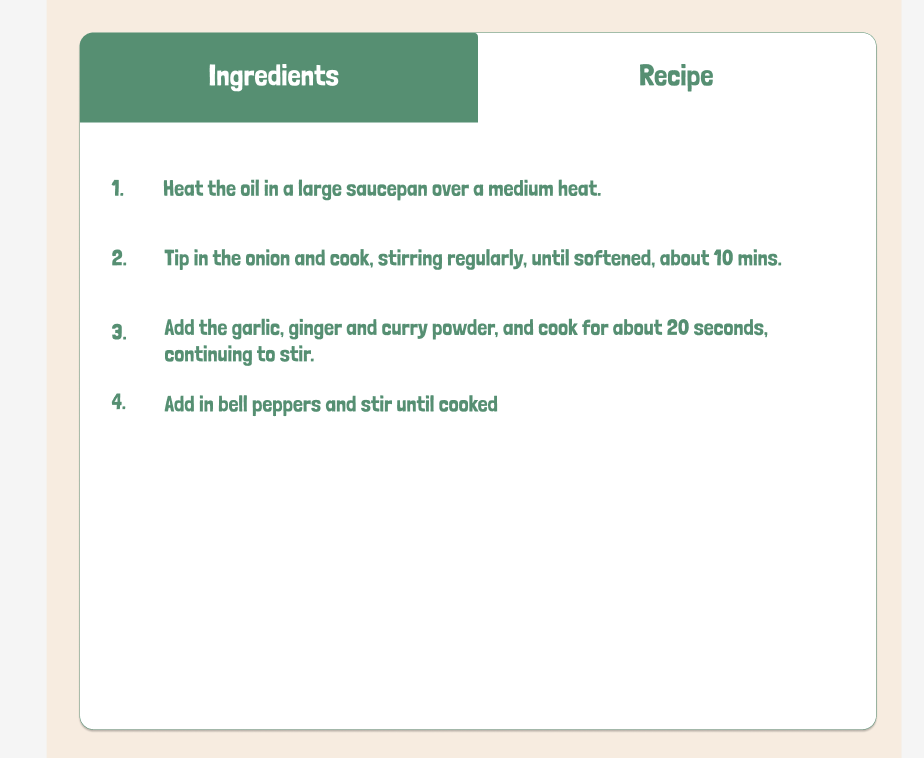
\includegraphics[width=1.0\textwidth]{assets/design-images/Version 1 Recipe Switcher recipe.png}
  \centering
  \caption{Recipe Switcher component design showing recipe instructions}
\end{figure}

\subsubsection{Designs: Version 2}
The second iteration of our designs focused more on user experience and frontend features, aiming to further elevate the overall usability and engagement of our web application.

Within this version, we added an add recipe form to allow users to add in their own recipe into the system, as well as a homepage menu and back buttons to increase navigation across the application. We also reviewed some of the components and features that we designed from version 1, and removed any features we thought we no longer needed.

\paragraph{Add Recipe Form}
After discussing what features could be added to the application, we found that one of the most impactful addition would be to have an “Add Recipe” form. This form would allow users to add in their own recipes to the system so we could diversify recipes more to the users taste whilst also giving them the same step by step functionality shown within the recipe carousel.

Initially, we created two different designs for the form. Both forms featured buttons which were would toggle between different forms, each corresponding to the heading of the respective button.

Within Design 1, the buttons were positioned on the left-hand side of the page, while the corresponding forms were located on the right-hand side. Design 2 incorporated a 'recipe switcher' component, with form boxes situated below the corresponding headings.

After a few discussions, we decided that the layout of Design 2 provided a more user-friendly experience. Since this component was already featured elsewhere within the application, we opted for consistency and familiarity by incorporating it into the form design as well.

\begin{figure}[h]
  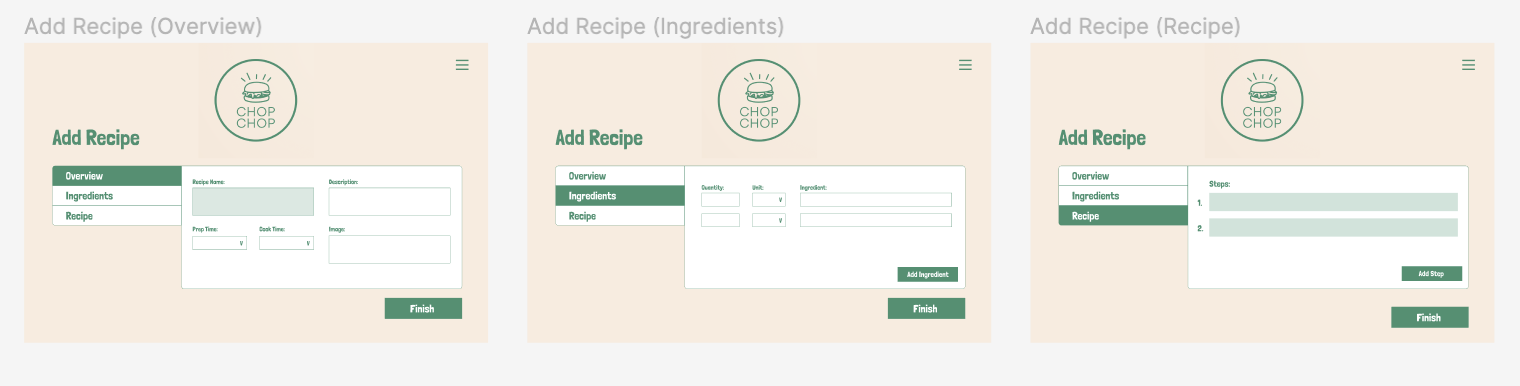
\includegraphics[width=1.0\textwidth]{assets/design-images/Design 1 Add Recipe Form.png}
  \centering
  \caption{Add Recipe form: Design 1 }
\end{figure}

\begin{figure}[h]
  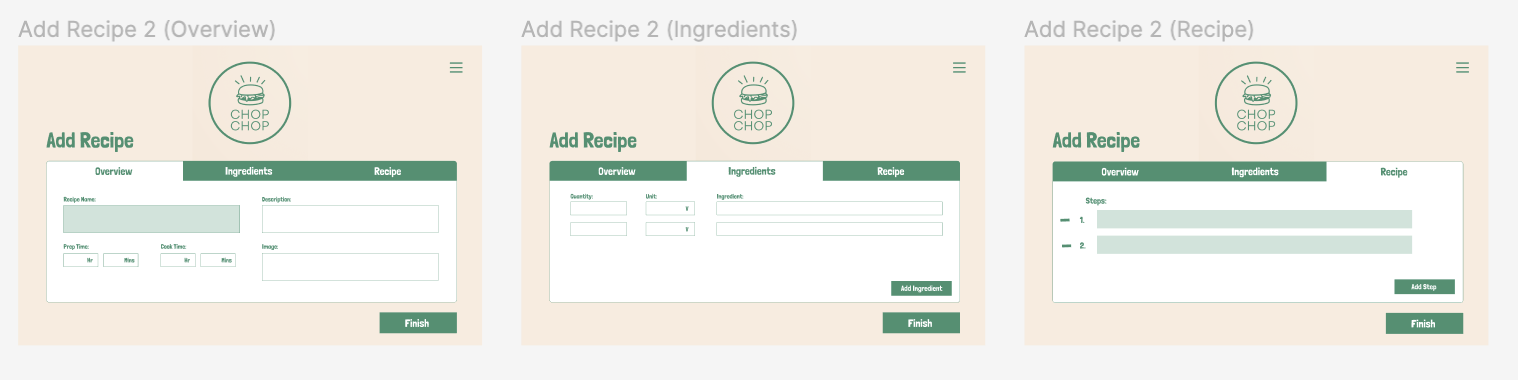
\includegraphics[width=1.0\textwidth]{assets/design-images/Design 2 Add Recipe Form.png}
  \centering
  \caption{Add Recipe Form: Design 2}
\end{figure}

\paragraph{Navigation Menu}
To improve user experience within the application, we decided to add a navigation menu to the application, which would act a centralised hub to important links. By implementing this menu, we hoped that it would streamline user journey, enhance usability and lead to a increased user satisfaction.

\paragraph{Back Buttons}
Upon review of the version 1 designs, we noticed that there was not a clear way for users to navigate around the application. The original idea was to have our logo as the main way to access the homepage, and as the application had shallow page structure, we did not see the need for a back button except for when navigating on the recipe carousel page.

Within version 2 of the design we introduced a new homepage menu and expanded the number of pages within the application. This added an importance to provide users with a clear way to navigate and enhance their browsing experience. 

\paragraph{Downfalls}
Between Version 1 and 2 of the designs, there was not many features which we removed. We mainly focused on refining and optimising existing features, as well as introducing new elements to enhance usability and overall user experience.

However, we decided to remove some unnecessary features to reduce clutter within the application and enhance user experience. The first feature which we deemed redundant was within the recipe switcher component. Originally, we wanted to add a checkbox for users to select if they had already prepared ingredients for the recipes. For instance, if they had already chopped carrots in advance, they could mark this checkbox to skip over related steps within the recipe carousel page. However, we realised that this would this would add unnecessary complexity to the user interface and potentially confuse users.

We also removed the idea of implementing tags within recipes and recipe cards. We found that this would make the database overly complex and potentially overwhelming for users to navigate. The metadata shown for recipes were also not essential for the core functionality of the application, so to simplify the design we opted to eliminate this feature.


    \subsection{Architecture}
    \subsubsection{Software}
    Due to the size and complexity of this project, we knew we needed to outline what we needed before begining a substantial ammount of work. First, we detailed what we wanted: a multi-platform app capable of identifying and progressing steps of a recipe. We then researched how we could execute our idea; we settled on a basic client/server approach using a client, a server, and a database (which only the server could access). This would comprise the basis of our tech stack.

    \begin{figure}[t]
      \centering
      \begin{subfigure}{0.45\linewidth}
        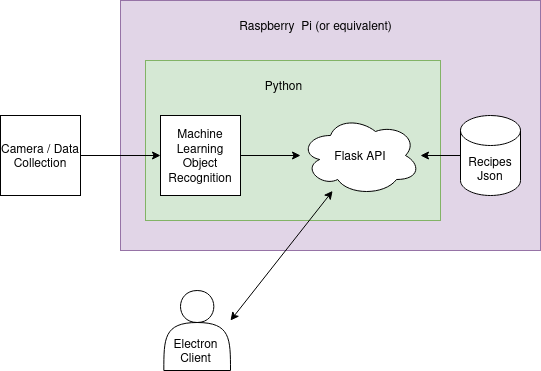
\includegraphics[width=\linewidth]{assets/first-architecture.png}
        \caption{}
        \label{fig:architectureA}
      \end{subfigure}
      \hfill
      \begin{subfigure}{0.45\linewidth}
        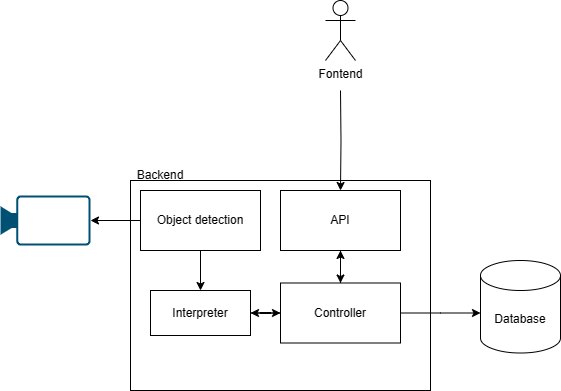
\includegraphics[width=\linewidth]{assets/second-architecture.png}
        \caption{}
        \label{fig:architectureB}
      \end{subfigure}
      \vfill
      \begin{subfigure}{0.5\linewidth}
        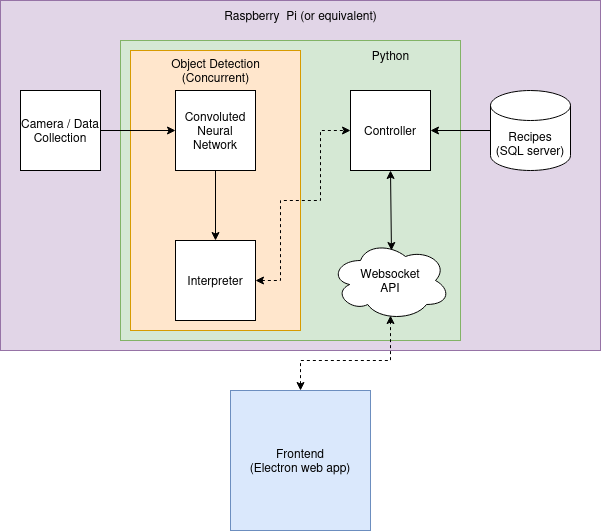
\includegraphics[width=\linewidth]{assets/final-architecture.png}
        \caption{}
        \label{fig:architectureC}
      \end{subfigure}
      \caption{Our architecture drawings in chronological order}
      \label{fig:architectures}
    \end{figure}

    In our first diagram (\ref{fig:architectureA}) we identified a very simplistic backend, it utilised a flask (REST) api to connect to the client and a backend without many control flows. There were cameras attatched to the backend and a database which the backend could also access.

    In our next drawing (\ref{fig:architectureB}), we detailed the backend control flow in-depth which helped us outline our python classes and files. We implemented a controller model where one central controller would process data and record the state of the program. This was to reduce complexity by making the code more modular.

    After much discussion, we decided to change our API to a websocket API to allow for multiple clients and two way communication. This also avoided the problem of long polling with a RESTful API.

    We also made our object detection system run concurrently so it could be interrupted or killed whit ease whilst still maintaining the API. Now, the controller and interpreter would send messages over python threads to communicate, like when a step has been detected or what step is next.

    Additionally, we changed our database from a JSON file to a relational databse (SQL Lite). This increased our application's scalability by allowing us to manage recipe data more easily rather than manipulating a plain-text JSON file.

    As a team we had lots of collaboration on the architecture, we would often draw up designs on whiteboards and discuss the pros and cons of each approach this led to us being well prepared for problems and making an architecture that is modular by design.\footnote{Figure \ref{fig:architectureC}, is not technically the final architecture diagram as we also added the multimedia gallery (section \ref{multimediaGallery}) which adds another database sending information to the frontend.}

    The planning of architecture contributed a lot to our process it allowed us to develop features simultaneously knowing how they would interact ahead of time.

    \subsubsection{Hardware}
    For the hardware, we looked into running our main backend on a Raspberry Pi with web-cameras connected via USB. The Raspberry Pi would host the websocket API on our local network for any devices using the frontend to connect to. An SQL Server would also be hosted on the Raspberry Pi locally for it to access.

    This way of hosting made it easier to debug as we could 'fake' messages from the frontend or backend using HTTP requests. 

    In reality, the Convoluted Neural Network ran inneficiently on the Raspberry Pi so we substituted it for a normal laptop, however, our modular architecture allowed us to do this with no problems.

    \section{Development}
    \subsection{Backend}
        The backend is divided into several sections: API, controller, interpreter, and object detection. Additionally, we have utilities and tests, which support and are utilised within other sections. The backend is initiated from \verb|main.py|, which launches the controller, API, and our logging system, producing two separate log files: one called \verb|detection| and one called \verb|API| to help us track the status of the program. We also have \verb|config.py|, which houses common variables used throughout the backend. This allows us to easily change any of these variables without delving too deeply into the backend.
    \subsubsection{Controller}
    Our controller keeps state for the backend: storing the current recipe and step, taking messages from the API to the database, and handling detection events from the interpreter. It is built from 3 core scripts, the Controller main script, a manageThread script and a recipe script. 
    
    The recipe script is for all the getter and setter functions that are recipe dependent. This includes functions such as \verb|get_command_for_step()| to be able to read and serve the human readable commands to the frontend and \\ \verb|get_progression_requirements_for_step()| to get and serve the progression objects to the interpreter. We split these functions into a separate script from the main Controller as they are recipe dependent, meaning we need to have already selected a recipe in the initialisation stage of this script and we wanted to keep this function out of the main controller script as that also houses recipe independent functions.
    The main Controller script contains functions for starting new recipes, recipe dependent functions called from the recipes script and recipe independent functions such as retrieving all recipe metadata for displaying multiple recipes on the frontend.
    \subsubsection{Interpreter}
    The interpreter acts as a link between the visual inputs coming out of object detection and the controller, it operates on a separate thread, allowing the controller to handle frontend requests simultaneously and without interruption. We initialise the interpreter thread with the progression object, inhibitor object and camera passed into it, this setup enables the interpreter to query the object detection module for the presence of progression objects while ensuring the absence of inhibitory ones. Additionally, we add hands as a default inhibitor object to ensure that the interpreter does not progress while the user is still working on the current step. Hard coding this into the interpreter reduces the need to specify them for each individual step and avoids clogging up the database with duplicate information.
    
    Instead of initialising the cameras inside the interpreter, which was our initial approach, we now initialise them outside of the thread in an initialisation script and pass them into the interpreter. This change was made because the initial method led to long processing time between recipe steps as each step required the cameras to be reinitialised as a new thread was being created. With this change the progression between recipe steps significantly sped up, with the trade-off being that it now takes slightly longer to initialise the recipe at the beginning.
    
    To help prevent false positives from progressing the step prematurely we implemented a rolling average process into the interpreter. To achieve this we developed a custom \verb|LimitedQueue| datatype. This datatype is used to take an average over the last 10 outputs from object detection as true or false denoting whether the last frames met progression the requirements, with at least 6 of these frames needing to be true to allow the step to progress. We experimented with the number of frames being used to calculate our rolling average and found that 7 out of a set of 10 worked well to reduce the false positives without significantly delaying progression times. This was easy to experiment with as both these variables are housed inside \verb|config.py|.
    
    Once the rolling average requirement is met, the thread closes, triggering an \verb|'end_thread'| function that isn’t run on the thread itself. This function informs the controller that the step has been completed and progresses the step sending a message to the API for the frontend and starting a new thread with the progression and inhibitor objects for the next step.

    \subsubsection{Object Detection}
    The object detection module is designed to analyse individual frames for the presence of progression and inhibitory objects. When queried by the interpreter, it captures the current frame using OpenCV2 and processes it using Supervision and  Ultralytics libraries to extract tags for the objects visible in the frame. Subsequently, it determines whether progression objects are present in the list and inhibitory objects are absent, returning either true or false accordingly.
    \subsubsection{API}
    Our project's API system comprises two main components: a WebSocket server and a custom HTTP server. These two systems run at the same time to achieve different parts of the API requirements.
    
    \paragraph{WebSocket Server}
    The WebSocket server facilitates real-time bidirectional communication between clients and the server, operating on asynchronous principles. It consists of two main handlers: a consumer and a producer. The handler function serves as a central component, running both consumer and producer handlers using the asyncio library to run at the same time.
    
    The consumer handler processes incoming requests from clients, parsing JSON payloads into request objects, and executing corresponding commands. These commands involve interactions with the controller or the database.
    
    The producer handler manages outgoing responses to clients, continuously monitoring changes in the system state. For instance, it tracks updates in recipe steps and broadcasts these updates to all connected clients. 
    
    \paragraph{Custom HTTP Server}
    The custom HTTP server handles file retrieval and uploads from the multimedia gallery. It extends the \verb|MyCustomHTTPRequestHandler| class, inheriting functionality from Python's \verb|http.server.SimpleHTTPRequestHandler|.
    
    Its primary function is to retrieve multimedia content, such as photos or voice lines, from the gallery via URLs. If it receives a POST request, the server validates whether the request contains image data. If image data is present, the server stores the uploaded image in the Multimedia Gallery.
    
    \subsection{Frontend}
    \subsubsection{Vue.js}
    Whilst researching for the frontend we considered a number of different frontend frameworks before settling on Vue.js (vue), Node.js (node), and electron. We had discussed using Flutter as opposed to vue since it's superiour at making mobile interfaces however, as making a mobile app became less prioritised we decided to go with vue for the following reasons: 
    \begin{description}
      \item[Flexibility:] vue is flexible, we can make custom components to fit our application, we can test it on a web-browser and utilise powerful debuging tools, additionally with a bit of work we can sandbox it into a mobile application.
      \item[Easy to learn:] vue's syntax and component systems are easy to learn and to read which suits our team, some of which had never used a frontend framework before. This makes understanding the code much easier when it comes to reviewing merge requests or discussing approaches.
      \item[Lightweight:] vue is lightweight, it's quick to load as it is made to be run from a web-browser. Features like hot reload help us devlop quickly and it's cli tools\footnote{in addition to the node package manager} make installing packages easy.
      \item[Familiarity:] our team already had some experience in vue so it would be quicker to develop with and easier to teach to other team memebers.
    \end{description}

    \subsubsection{SCSS}
    
    \subsubsection{BEM coding standards}
    The BEM (Block Element Modifier) methodology is a popular naming convention for classes in HTML and CSS. Its goal is to help developers better understand the relationship between the HTML and CSS in a given project. 

    We decided to use the BEM methodology within our project to maintain consistency and improve code readability. By adopting this naming convention, we felt like we could manage and differentiate between components and their corresponding styles creating a more robust and maintainable codebase. 
    
    The use of modifiers allowed us to reuse code within the project, while also providing a way to add customisations to existing components. 

 
    \subsection{Database}
    \subsubsection{JSON}
    We originally built a JSON database to quickly get started with storing recipes. We broke the initial database into separate recipes, each with three distinct areas. Recipe Details contained the recipe ID, Name and Description, Recipe Ingredients contained all the ingredient Names as well as Amount and Unit. Recipe Steps then contained Steps in human readable form, the Progression Object and Inhibitor for the backends understanding and the Camera which the step is expected to be completed under.
    
    We chose to use JSON to start with due to its quick and simple nature to set up, allowing us to quickly begin testing the process of displaying recipe details and ingredients on the frontend and progressing through recipe steps with the backend.
    
    When breaking the recipes into separate steps we knew we had to do it in a way that could be easily translated into Progression Objects and Inhibitor Objects. From our first database we had the steps broken down into their most simple form so that the neural network would only ever have one object to be looking for at once. It was important that this step was done early as it led the way for knowing what images we would need to have for our training dataset.
    \subsubsection{SQL}
    Further into the project, once we had a good setup for displaying and progressing our recipes, we wanted to add a significant amount of “dummy data” to fill out the frontend application and allow for features such as featured recipes and recipe searching. It became clear that the JSON database would no longer be the best way to store our recipes and we instead opted to transition to an SQL database before progressing with adding the additional recipes and search functionality.
    After deciding to migrate to an SQL database, we conducted research and opted for SQLite over other SQL database engines. This choice stemmed from our desire for a straightforward implementation while still leveraging the features of SQL and not needing to start running any more servers which would have been required for an SQL server.
    
    The SQL database comprises five tables, three of these tables are mapped from the same segments that were split from the JSON data. These tables include Recipes, which store core recipe information such as name and description, Steps which is linked to recipes in a one-to-many relationship, and Ingredients, also linked to recipes in a one-to-many relationship. Recipes contains the same information as it did in the JSON, while Steps and Ingredients needed a column added for RecipeID to now be able to link it back to the recipe they belong to.
    
    Additionally, the database includes two new tables to accommodate the work done with voices. The Voices table assigns a unique ID to each voice, and the Recipe\textunderscore Voices table facilitates many-to-many connections between recipes and voice recordings.
    \subsubsection{Multimedia Gallery}\label{multimediaGallery}
    As well as the SQL database the final project also contains a file storage server to store our photos and voice recordings for recipe steps. This is local file storage server with its location stored inside the SQL database.
    
    This file storage is called using a custom HTML web request to retrieve the images and voice recordings. We chose to store our recipe images like this as we found it to be the simplest and easiest way to store photos with a focus on scalability.

    \subsection{Data Collection \& Training}
    \subsubsection{RoboFlow}
    For developing our object detection system, we needed a trained model. From our research, we decided to use Roboflow for data collection and management and trained with YOLOv8.
    
To train, we first needed to collect many images of the object we wanted to detect. We found during development that it is best to start with lots of good-quality images of the object; They should be in good lighting and well-framed. Then many different positions of objects in the frame. Finally, gathering some more obscure images. These can be in different lighting conditions, from far away, and with multiple other objects in the frame as well. These all create a diverse data set, which increases the chance of detection.

Once a significant number of images had been gathered (around 100) they were uploaded to Roboflow for annotating. Annotation jobs can be generated and sent to each person on the project. We decided to use box annotation, as it was significantly quicker to annotate and in our preliminary tests offered the same level of object detection that poly-selection did.

Each annotation was then reviewed by someone else before being added to the dataset. This ensured that the dataset was accurate in its annotations as small mistakes could teach the AI the wrong classification.

When all images are annotated a new YOLOv8 dataset can be generated. Before this Roboflow will split up your images into training, testing, and validation. Training will teach AI, validation are used to as it trains test how good the AI is getting. Testing “a test data set is a separate sample, an unseen data set, to provide an unbiased final evaluation of a model fit.” \cite{trainvalidtest} It will resize the image to 640x640 which greatly reduces training time, and smaller images reduce computational cost. 

Finally, it generates extra images through augmentation. We chose Shear ±15° and Brightness ±25\%. Shear would simulate different camera angles, which would provide greater angle coverage. Brightness would widen the number of handled lighting conditions, as different kitchens could have very varied levels of brightness.

    \subsubsection{Training YOLO with CUDA}
    While RoboFlow did offer the option to train the models for us, it required monetary payments, so we opted to train on our Nivida GPU using CUDA \cite{cudacuda} instead.

    CUDA allows for faster YOLO training. It works by taking advantage of CUDA cores that are found on Nivida Graphics cards. In short “CUDA is NVIDIA’s parallel computing architecture. It enables dramatic increases in computing performance, by harnessing the power of the GPU” \cite{ghorpade2012gpgpu}. YOLO itself uses Pytorch \cite{nvidiapytorch} which implements tensor cores, “similar to a multidimensional array, used to store and manipulate the inputs and outputs of a model, as well as the model’s parameters. Tensors are similar to NumPy’s ndarrays, except that tensors can run on GPUs to accelerate computing” \cite{nvidiapytorch}. 
    
    By running this command we were able to train our model
    \begin{verbatim}
    yolo task=detect \
        mode=train \
        model=yolov8s.pt \
        data={Location-Of-Dataset}/data.yaml \
        epochs=100 \
        imgsz=640 \
        device=0
    \end{verbatim}


    Which took in the dataset (data.yaml) from RoboFlow, and outputted weights, and results of the training.


    \subsubsection{Reviewing \& Improving}


    \begin{figure}[htbp]
        \begin{minipage}[htbp]{1\linewidth}
            \centering
            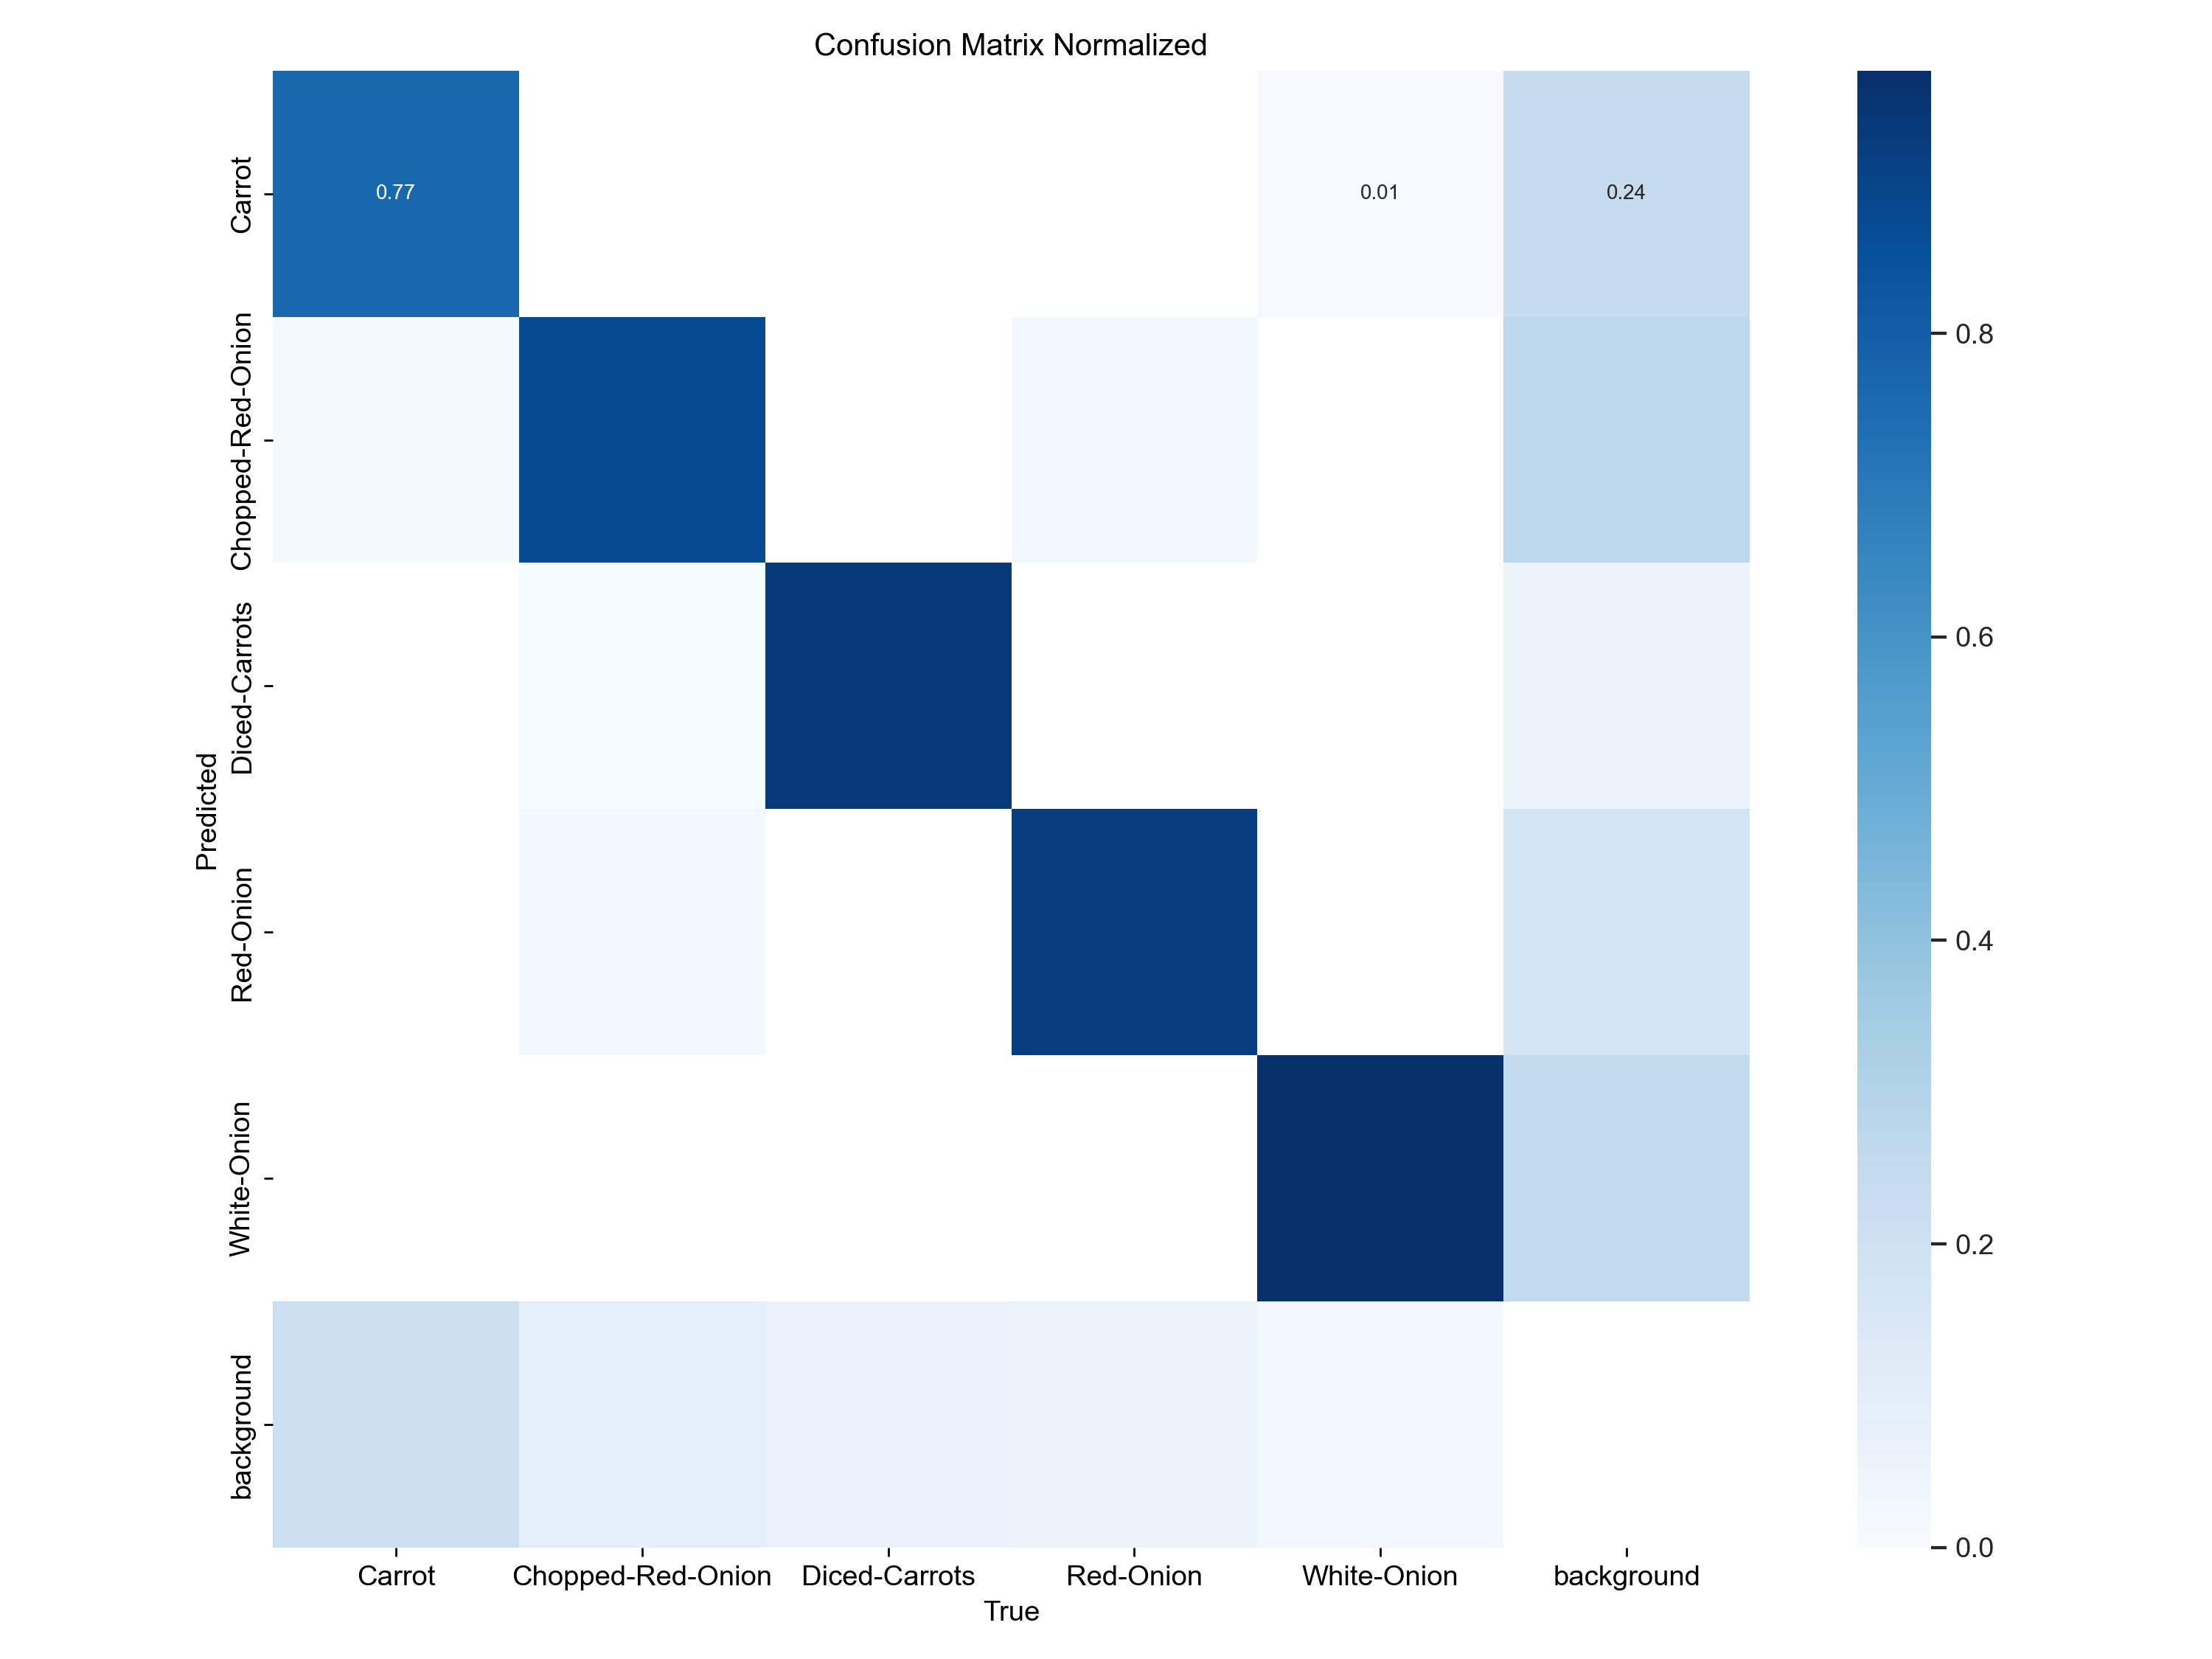
\includegraphics[width=\linewidth]{assets/confusion_matrix_normalized-Version-1.png}
            \caption{Confusion Matrix for first model (normalized)}
        \end{minipage}%
        
        \begin{minipage}[htbp]{1\linewidth}
            \centering
            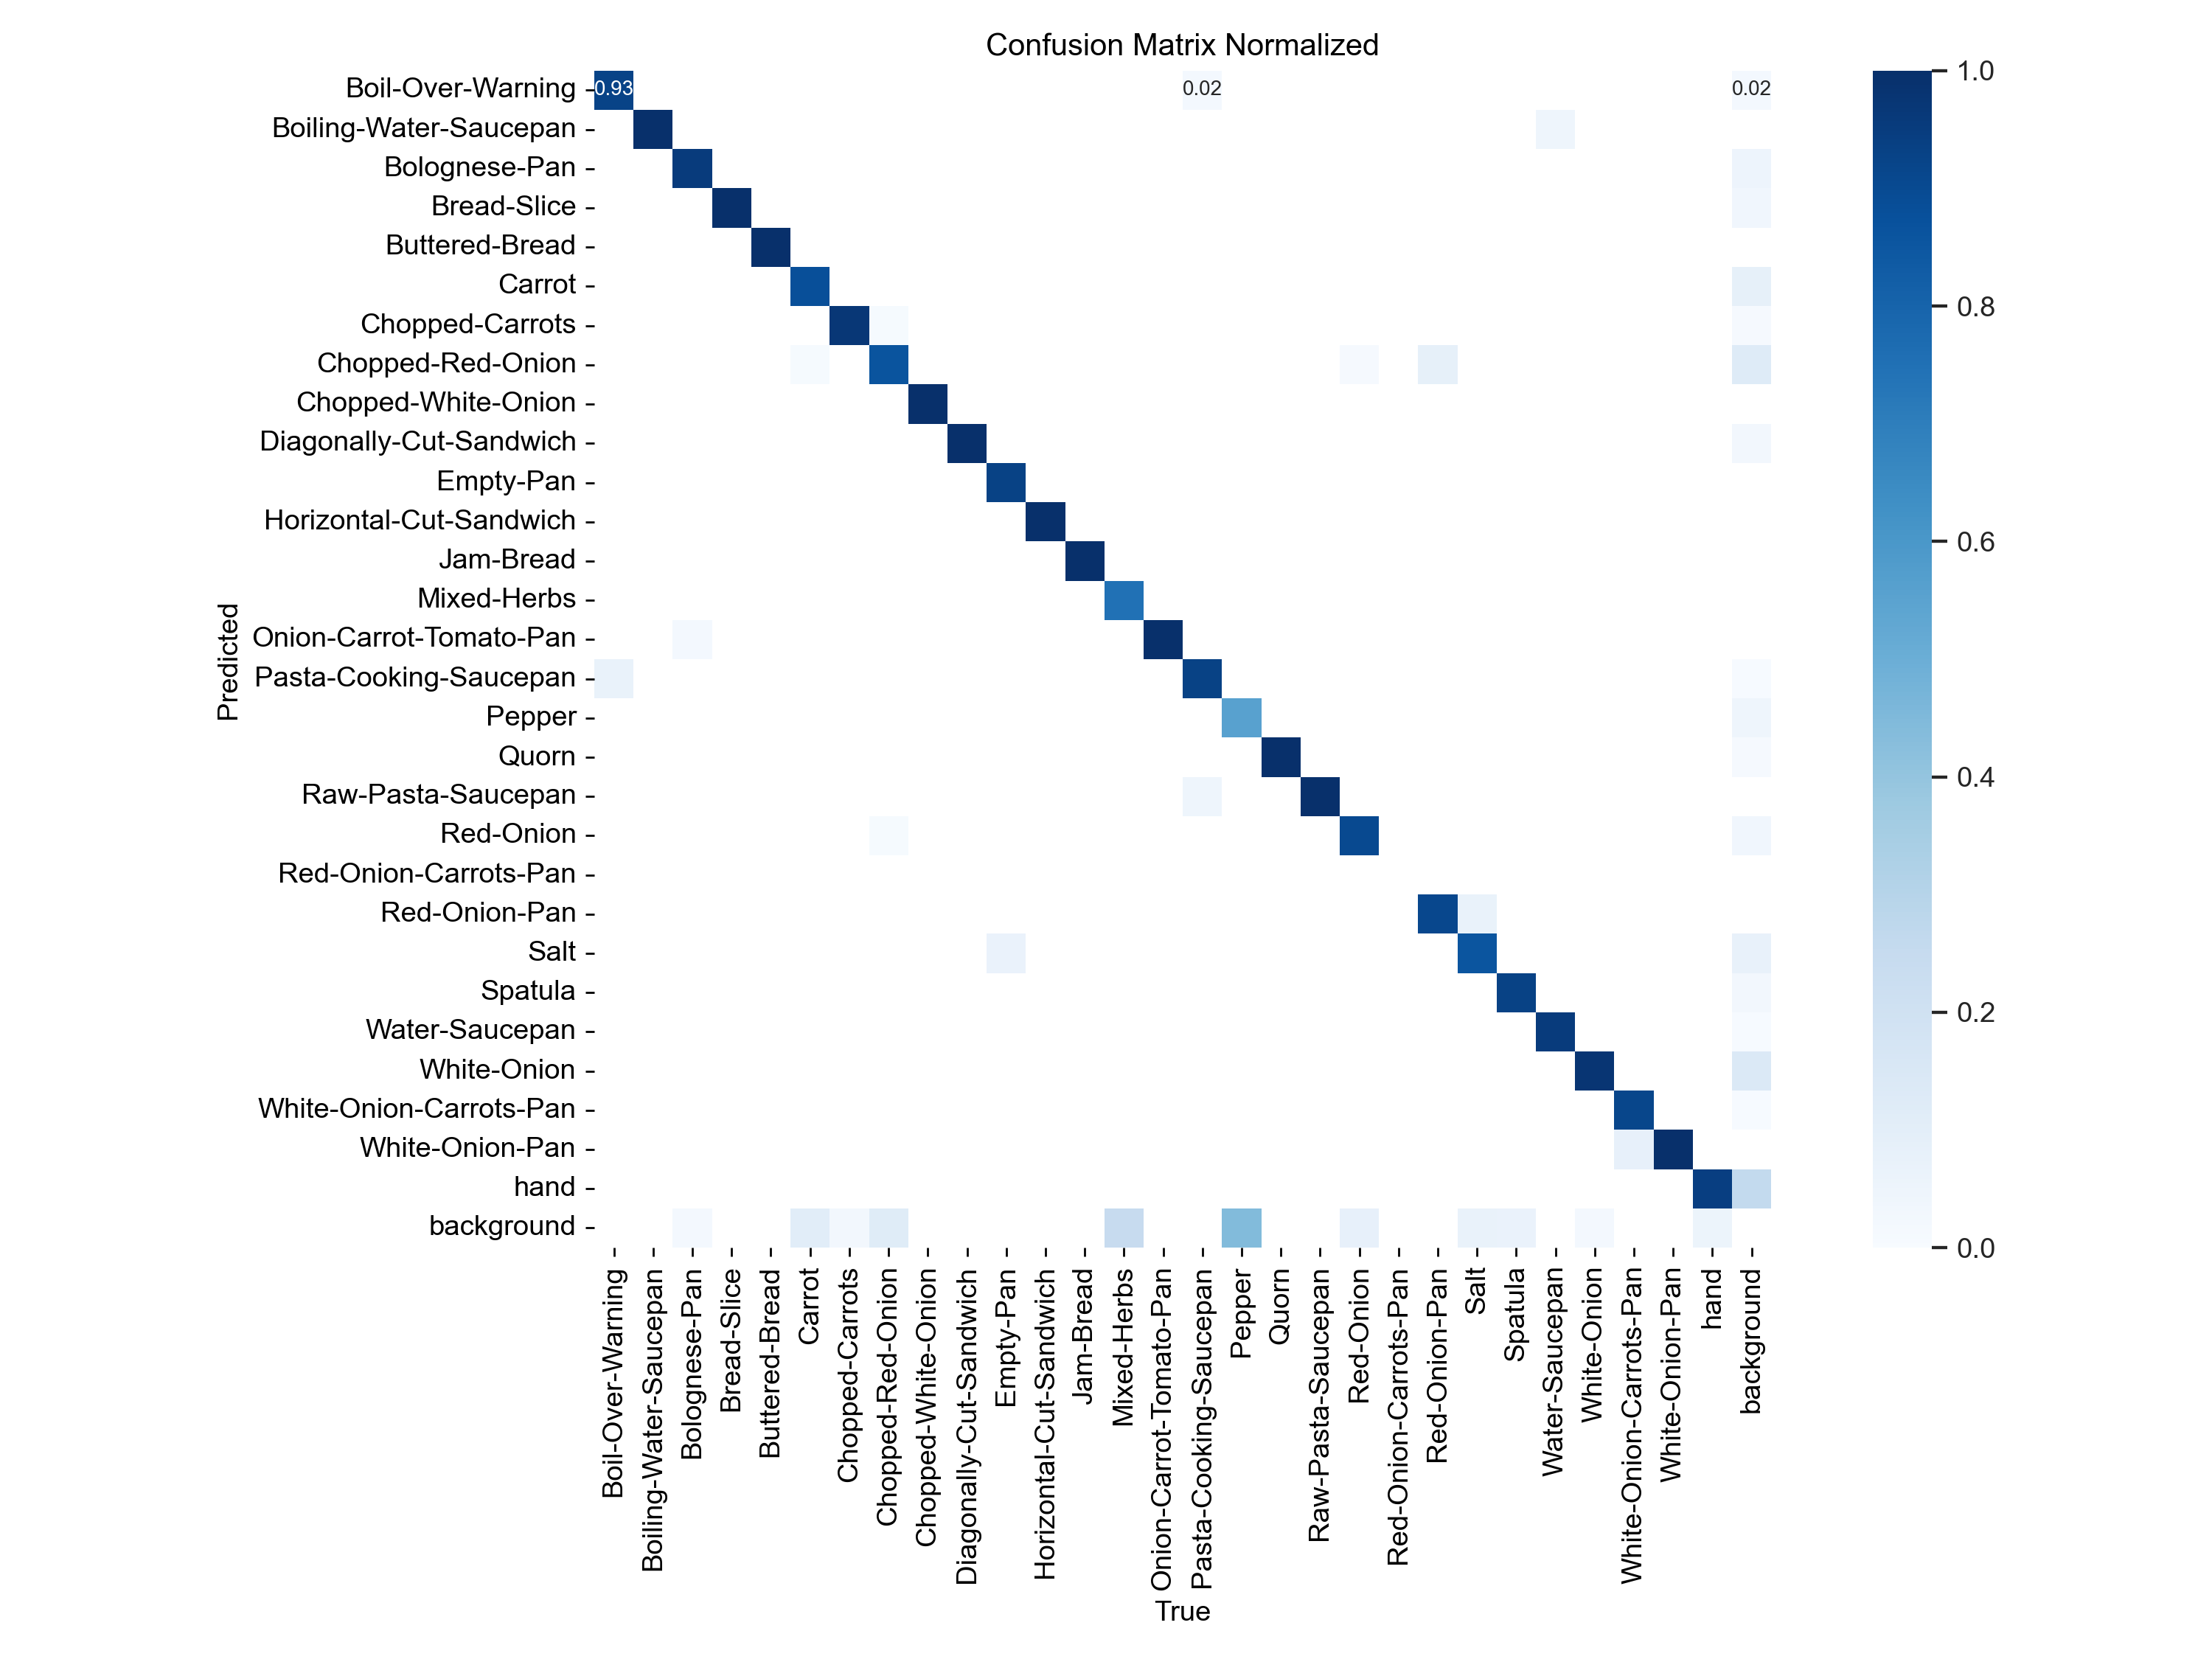
\includegraphics[width=\linewidth]{assets/confusion_matrix_normalized-Version-6.png}
            \caption{Confusion Matrix for last model (normalized)}
        \end{minipage}
    \end{figure}
    
    ////Here we will add graphs of our results for our first model and the last model showing how we improved over time

    Also, talk here about how we improved out data collection over time, also mention null data


    \section{Testing}
    ////This section we will talk about our attempts at recording a chop-chop video. Refer to youtube for this and also old recordings

    Maybe also talk about user testing from other people (friends)

    \section{Results}
    //// Talk about the success and also how well the poster fair went. Here is a great place to talk about reliability. Great place to also talk about the varied nMap-50 scores (hands are high other are not)

    \section{Future Work}
    //// TTS could be mentioned here along with accessibility, you could also include some blue sky thinking about how this would be included in side people kitchens.


    \section{Conclusion}
    //// Say it was a success, say what we didn't manage to do

    \pagebreak

    
  %\end{multicols}
  
  \addcontentsline{toc}{section}{References}

  \bibliographystyle{ieeetr}
  
  \bibliography{group-doc}

\end{document}